% Options for packages loaded elsewhere
\PassOptionsToPackage{unicode}{hyperref}
\PassOptionsToPackage{hyphens}{url}
%
\documentclass[
]{article}
\usepackage{amsmath,amssymb}
\usepackage{lmodern}
\usepackage{iftex}
\ifPDFTeX
  \usepackage[T1]{fontenc}
  \usepackage[utf8]{inputenc}
  \usepackage{textcomp} % provide euro and other symbols
\else % if luatex or xetex
  \usepackage{unicode-math}
  \defaultfontfeatures{Scale=MatchLowercase}
  \defaultfontfeatures[\rmfamily]{Ligatures=TeX,Scale=1}
\fi
% Use upquote if available, for straight quotes in verbatim environments
\IfFileExists{upquote.sty}{\usepackage{upquote}}{}
\IfFileExists{microtype.sty}{% use microtype if available
  \usepackage[]{microtype}
  \UseMicrotypeSet[protrusion]{basicmath} % disable protrusion for tt fonts
}{}
\makeatletter
\@ifundefined{KOMAClassName}{% if non-KOMA class
  \IfFileExists{parskip.sty}{%
    \usepackage{parskip}
  }{% else
    \setlength{\parindent}{0pt}
    \setlength{\parskip}{6pt plus 2pt minus 1pt}}
}{% if KOMA class
  \KOMAoptions{parskip=half}}
\makeatother
\usepackage{xcolor}
\usepackage[margin=1in]{geometry}
\usepackage{longtable,booktabs,array}
\usepackage{calc} % for calculating minipage widths
% Correct order of tables after \paragraph or \subparagraph
\usepackage{etoolbox}
\makeatletter
\patchcmd\longtable{\par}{\if@noskipsec\mbox{}\fi\par}{}{}
\makeatother
% Allow footnotes in longtable head/foot
\IfFileExists{footnotehyper.sty}{\usepackage{footnotehyper}}{\usepackage{footnote}}
\makesavenoteenv{longtable}
\usepackage{graphicx}
\makeatletter
\def\maxwidth{\ifdim\Gin@nat@width>\linewidth\linewidth\else\Gin@nat@width\fi}
\def\maxheight{\ifdim\Gin@nat@height>\textheight\textheight\else\Gin@nat@height\fi}
\makeatother
% Scale images if necessary, so that they will not overflow the page
% margins by default, and it is still possible to overwrite the defaults
% using explicit options in \includegraphics[width, height, ...]{}
\setkeys{Gin}{width=\maxwidth,height=\maxheight,keepaspectratio}
% Set default figure placement to htbp
\makeatletter
\def\fps@figure{htbp}
\makeatother
\setlength{\emergencystretch}{3em} % prevent overfull lines
\providecommand{\tightlist}{%
  \setlength{\itemsep}{0pt}\setlength{\parskip}{0pt}}
\setcounter{secnumdepth}{5}
\newlength{\cslhangindent}
\setlength{\cslhangindent}{1.5em}
\newlength{\csllabelwidth}
\setlength{\csllabelwidth}{3em}
\newlength{\cslentryspacingunit} % times entry-spacing
\setlength{\cslentryspacingunit}{\parskip}
\newenvironment{CSLReferences}[2] % #1 hanging-ident, #2 entry spacing
 {% don't indent paragraphs
  \setlength{\parindent}{0pt}
  % turn on hanging indent if param 1 is 1
  \ifodd #1
  \let\oldpar\par
  \def\par{\hangindent=\cslhangindent\oldpar}
  \fi
  % set entry spacing
  \setlength{\parskip}{#2\cslentryspacingunit}
 }%
 {}
\usepackage{calc}
\newcommand{\CSLBlock}[1]{#1\hfill\break}
\newcommand{\CSLLeftMargin}[1]{\parbox[t]{\csllabelwidth}{#1}}
\newcommand{\CSLRightInline}[1]{\parbox[t]{\linewidth - \csllabelwidth}{#1}\break}
\newcommand{\CSLIndent}[1]{\hspace{\cslhangindent}#1}
\usepackage{setspace}\doublespacing \usepackage{lineno} \usepackage{placeins}
\usepackage{booktabs}
\usepackage{longtable}
\usepackage{array}
\usepackage{multirow}
\usepackage{wrapfig}
\usepackage{float}
\usepackage{colortbl}
\usepackage{pdflscape}
\usepackage{tabu}
\usepackage{threeparttable}
\usepackage{threeparttablex}
\usepackage[normalem]{ulem}
\usepackage{makecell}
\usepackage{xcolor}
\ifLuaTeX
  \usepackage{selnolig}  % disable illegal ligatures
\fi
\IfFileExists{bookmark.sty}{\usepackage{bookmark}}{\usepackage{hyperref}}
\IfFileExists{xurl.sty}{\usepackage{xurl}}{} % add URL line breaks if available
\urlstyle{same} % disable monospaced font for URLs
\hypersetup{
  hidelinks,
  pdfcreator={LaTeX via pandoc}}

\author{}
\date{\vspace{-2.5em}}

\begin{document}

\setcounter{page}{6}

\begin{center}
    
\textbf{\Large Using mechanistic models to assess temporary closure strategies for small scale fisheries}
    
\textsc{Sophie Wulfing$^{1*}$, Ahilya Sudarshan Kadba$^{1}$, Mez Baker-Médard$^{2}$, and Easton R. White$^{1}$}
\vspace{3 mm}
\normalsize{\indent $^1$Department of Biological Sciences, University of New Hampshire, 03824, NH, USA \\ $^2$Department of Environmental Studies, Middlebury College, Middlebury, VT 05753\\}
$\text{*}$ Corresponding authors: Sophie Wulfing (SophieWulfing@gmail.com) and Dr. Easton White (Easton.White@unh.edu)
\end{center}

\newpage

\linenumbers

\hypertarget{abstract}{%
\section{ABSTRACT}\label{abstract}}

Mechanistic models are particularly useful for understanding and predicting population dynamics in data deficient species. Data deficiency is a relevant issue in small scale fisheries as they are generally under studied and underrepresented in global fishing datasets. As overfishing remains a global issue, especially in small-scale fisheries, one commonly utilized conservation method is temporary closures. The blue octopus (\emph{Octopus cyanea}) fishery off the southwest coast of Madagascar is one such system that uses temporary closures, yet lacks sufficient data collection to assess the viability of the population. This fishery is a key economic resource for the local community as blue octopus catch is sold by local fishers to international and local export markets and is a major component of fisher income. To assess the sustainability of blue octopus, we parameterize a Levkovitch population matrix model using existing catch data. In this study, we show that this population was in a decline of 1.8\% per month at the time of data collection. To sustain the existing population of blue octopus, our model indicates that the fishery would need to close for at least three months annually. Increasing the length of closure is predicted to significantly increase the octopus population at these sites. We show that if implemented correctly, temporary closures could be used to restore this population. The local communities of Madagascar have implemented various fishing restrictions to ensure sustainable fishing, indicating a need for further research into the effectiveness of these fishing closures. Therefore, our study provides insight into the underlying population dynamics of this fishery and provides survivability estimates of this species.

Keywords: \emph{Octopus Cyanea}, matrix model, small scale fisheries, Madagascar, temporary closures

\hypertarget{introduction}{%
\section{INTRODUCTION}\label{introduction}}

Mechanistic models in ecology explicitly account for species life histories, behavioral, or other mechanisms to describe how a population or community may change over time (André, Haddon, and Pecl 2010; Briggs-Gonzalez et al. 2016). Mechanistic models can be important in situations without existing long-term data, when future conditions may not be similar to the past, and when different scenarios or actions need to be assessed (Crouse, Crowder, and Caswell 1987; Nowlis 2000; Gharouni et al. 2015). Thus, mechanistic models play a critical role in making informed conservation decisions, such as the management of small-scale fisheries.

Worldwide, 32 million fishers make their livelihood in small-scale fisheries, a subsector in which 90 to 95\% of fish is distributed for local consumption. These marine products are a vital source of nutrition for these communities ({``Hidden {Harvest}-{The} {Global} {Contribution} of {Capture} {Fisheries}''} 2012). The southwest region of Madagascar is one such area where subsistence fishing is an essential component to the diet and income of the local community. The ocean environments off the southwest coast of Madagascar are home to a wide variety of marine life, as sand beds, seagrass beds and coral reefs are all prominent biomes in the area. In fact, Madagascar has been calculated as a country that would benefit greatly from marine conservation given its economic reliance on marine harvests and the fact that it is a refuge to many marine species (Laroche et al. 1997). In the early 2000's, however, Madagascar began to move from local, subsistence fishing to also selling catch to export markets (Humber et al. 2006). There is evidence that up to 75\% of all fish caught in select villages is now sold to outside entities for international export (Baker-Médard 2017).

Locally-managed marine areas (LMMAs) are defined as coastal and near-sore fisheries in which resources are managed almost entirely by local communities and fishery stakeholders that live in the region. Because management is conducted by those directly affected by the fishery, goals typically include maintaining the livelihood and economic and cultural goals of the local community along with environmental goals (Govan 2010). LMMAs have grown in popularity among conservationists in small scale fisheries due to this empowerment of local fishers. Because of this, LMMAs tend to have greater local participation and compliance from stakeholders when compared to top-down regulation from governing bodies (Katikiro, Macusi, and Ashoka Deepananda 2015). LMMAs have been shown to improve both fisheries and fisher livelihoods in Kenya (Kawaka et al. 2017), Pacific Islands (Govan 2010), and in Madagascar (Mayol 2013). In Madagascar, the use of LMMAs has increased significantly since 2004, and fishers in the country have seen significant improvements to fish stocks as well as have experienced economic benefits since (Benbow and Harris 2011; Gilchrist et al. 2020). In order to protect fishing resources, Madagascar has instituted various conservation programs. Marine Protected Areas (MPAs) are regions in the ocean identified as being biologically important and fishing protections are therefore enforced. Before their establishment in Madagascar, governmental bodies had bans on certain types of fishing gear, implemented seasonal fishing regulations, and criminalized the harvest of endangered species. However, these strategies proved ineffective in execution and in their conservation goals (Humber et al. 2006). Both the government and nongovernmental organizations have since pledged to drastically increase the number of regions dedicated as MPAs through temporary fishing closures (Cinner et al. 2009; Oliver et al. 2015; Baker-Médard 2017).

One such class of MPAs that are currently being used in Madagascar are seasonal closures. These types of reserves have a long history of use and have been seen to successfully rehabilitate stocks (Camp, Poorten, and Walters 2015; Gnanalingam and Hepburn 2015). For example, seasonal closures have been shown to be an effective conservation strategy in increasing biomass the Atlantic sea scallop fishery in the United States (Bethoney and Cleaver 2019), restored natural trophic interactions in coral reef fisheries in Kenya (McClanahan 2008), and successfully restored the marlin stocks in Baja California (Jensen et al. 2010). This method is flexible, logistically simple for fishers and managers to understand, and mitigates the financial loss from the fishery that can be seen with permanent closures (Nowlis 2000; Humber et al. 2006; Cohen and Foale 2013; Camp, Poorten, and Walters 2015; Gnanalingam and Hepburn 2015; Oliver et al. 2015). However, seasonal closures are not always effective in their goal of replenishing stocks and this can depend on a wide range of factors. Ecological considerations about the life history of the target species, Allee effects, and changes to community structure and species interactions all play a role in how well the seasonal closure will protect the fishery (Russ and Alcala 1998; Cohen and Foale 2013; Gnanalingam and Hepburn 2015; Gilchrist et al. 2020; Grorud-Colvert et al. 2021). Further, the characteristics of the fishery itself has been seen to influence fishery recovery. Fishing method, where the effort will be redistributed to, and fishing activity upon reopening have all been factors in negating the recovery made during the closure (Hiddink et al. 2006; Humber et al. 2006; Cohen and Foale 2013). Therefore, assessments of each seasonal closure is essential to insuring that they are effective in replenishing fish stocks. Mechanistic modeling allows us to simulate different fishery scenarios and assess how populations will respond to these changes in fishing pressure.

Since 2003, when this marine resources in Madagascar first began to globalize, cephalopods have become one of the largest classes of exports (Humber et al. 2006; Aina 2009; Barnes-Mauthe 2013). This has since added significant fishing pressure to Madagascar's cephalopod populations and yield from this fishery has decreased in regions of this island such as the southwest Andavadoaka region (Humber et al. 2006). Cephalopods are a vital part of many ocean ecosystems and, compared to other fisheries, have a unique life history that can lead to distinct and variable population dynamics. Cephalopods act as both predators and prey in an ecosystem (Rodhouse and Nigmatullin 1996; Santos, Clarke, and Pierce 2001; Vase et al. 2021), situating them in a key role in food webs. They also provide rich nutrition and bioactive compounds to the oceanic microbial community (Fitahia et al. 2018). Further, their abundance varies drastically with a wide range of ocean conditions including sea surface and bottom temperature, salinity, currents, and sediment type (Catalán et al. 2006; Ibáñez et al. 2019; Van Nieuwenhove, Ratsimbazafy, and Kochzius 2019). Compared to other exploited marine organisms, cephalopods have a short lifespan coupled with a fast reproduction rate and high fecundity. This explains their population's ability to quickly bounce back when short term MPAs are introduced into their habitat (Humber et al. 2006; Katsanevakis and Verriopoulos 2006; Benbow et al. 2014). However, once fishing resumes, populations can suddenly and rapidly decline although in some examples, this could be attributed to heavy fishing pressure in the area right after reopening (Humber et al. 2006). Cephalopods are therefore extremely sensitive to both protection and harvest levels, and understanding how these volatile population dynamics will react to changes in fishing pressure is a key component to effective conservation of this resource.

\emph{Octopus cyanea}, or blue octopus, is the most abundant cephalopod species in the western Indian Ocean and is caught in about 95\% of local landings in Madagascar (Humber et al. 2006; Oliver et al. 2015). Like other cephalopod species, very little is known about their life history including natural death rate, larval survivability, and how much time this species remains in each stage of maturity. Further, age is difficult to determine from size alone as they have variable growth rates up to maturity (Wells and Wells 1970; Heukelem 1976; Herwig et al. 2012; Raberinary and Benbow 2012). Size limits have been shown to be the most effective method of conservation for cephalopods in general as it ensures individuals will breed before being harvested (Nowlis 2000; Emery, Hartmann, and Gardner 2016). To protect this species, size limits have been imposed on blue octopus catch in Madagascar, but these regulations are difficult in practice, as the fishing method used to harvest octopus involves spearing the octopus's den and extracting the octopus from the den. Blue octopus therefore typically die before size can be assessed, so octopus too small for market sale are typically harvested for household consumption (Humber et al. 2006). Further, the relationship between size and maturity stage is not strongly correlated (Raberinary and Benbow 2012) and as a result, size restrictions wouldn't necessarily protect individuals ready to reproduce and would be difficult to implement in the field. Therefore, temporary closures have been shown to be a more practical method of octopus conservation in that they can replenish stocks while maintaining fisher income (Benbow et al. 2014). However, this requires a deeper understanding of the characteristics of \emph{Octopus cyanea} in this fishery in order to be properly instituted. Instituting effective temporary closures in octopus fisheries can be difficult due to their short lifespan, high mortality, and sensitivity to environmental conditions (Catalán et al. 2006; Emery, Hartmann, and Gardner 2016; Ibáñez et al. 2019; Van Nieuwenhove, Ratsimbazafy, and Kochzius 2019). Lack of field data and difficulty of enforcement has also been a challenge in octopus fisheries, especially in Madagascar (Emery, Hartmann, and Gardner 2016; Benbow et al. 2014). This indicates that a thorough understanding of the life history of \emph{O. cyanea} and the harvest methods employed by fishers is necessary to enact meaningful fishing restrictions. Currently, the octopus fishery in this region of Madagascar is closed for the three months between June and August on a yearly basis (Benbow and Harris 2011; Westerman and Benbow 2014) which was decided in 2011. In this paper, we will also assess how this duration of closure will affect \emph{Octopus cyanea} stocks.

In this paper, we have three goals: 1) we will fit a Levkovitch matrix to the limited available data on \emph{Octopus cyanea} populations in southwestern Madagascar, 2) as well as create a theoretical estimation of the species' life history traits in different stages of its development and 3) determine the frequency and length in which these temporary closures should take place to maximize population health of the fishery and maximizing catch for the local community.



\begin{figure}
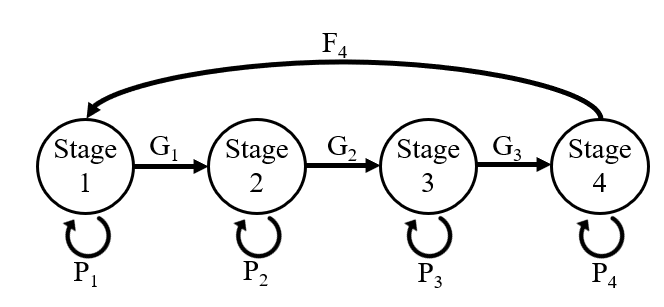
\includegraphics[width=0.45\linewidth]{LifeGraph} 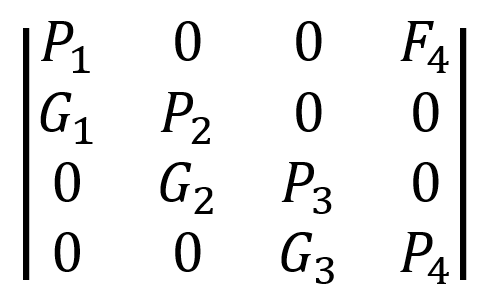
\includegraphics[width=0.45\linewidth]{MtxGeneric} \caption{A graph representing the life history of \emph{O. Cyanea} and the subsequent Lefkovitch Matrix where i corresponds with each of the stages of maturity (Immature, Incipient Mature, Mature, and Fully Mature individuals, respectively). \(P_i\) corresponds to probability of surviving and staying within a stage. \(G_i\) is the probability of surviving and growing to the next stage. \(F_i\) is the reproductive output of stage i. \label{LifeGraph}}\label{fig:LifeGraph}
\end{figure}

\hypertarget{methods}{%
\section{METHODS}\label{methods}}

As \emph{O. cyanea} has an extended larval phase and there is no existing data on the age structure of this population of octopus, we will use a stage-based population matrix, otherwise known as a Lefkovitch matrix (Caswell 2001). Here, the life history of the study organism is grouped by stages (Figure \ref{LifeGraph}), where each unit of the matrix represents a distinct period of the organism's life where it is subject to different environments, pressures, or physical attributes that would alter the survival and reproductive output at that phase, but the amount of time between each stage is variable. This would simply create different inputs for the probability of remaining in the same stage, and the growth and fecundity inputs can be based on available data. Lefkovitch matrices have not yet been applied to \emph{Octopus cyanea} populations and therefore could be a useful methodology to understand the dynamics of this population in the western Indian Ocean to better inform management strategies.

\hypertarget{data}{%
\subsection{Data}\label{data}}

To inform our model, we used data collected by Raberinary and Benbow (2012) from landings ranging from the villages of Ampasilava in the south to Andragnombala in the north which spans about 30 kilometers of coastline. Here, fishers usually fish along both reef flats and deeper barrier reefs. Fishers bring catch onshore either for household consumption or to sell to buyers for international export. This study collected landing data from February 2005 to February 2006 through daily surveying fishers as they landed onshore within a two hour window. They separated each octopus into five age classes: immature, incipient maturity, maturity, full maturity, and post laying. In this paper we omitted stage five, post laying, from this model as blue octopus only brood once, and stage five individuals therefore do not contribute to population growth. They recorded octopus weight, weight and length of gonads, sex, and a visual assessment of maturity class. A subsample of octopus were also collected for octopus length, and laboratory assessment of gonads for a confirmation of maturity class. They gathered this data on a total of 3,253 octopuses, and for the purposes of this study, we will be modeling from the 1,578 females collected. Despite there being no standardization for catch effort being available for this dataset, no other maturity stage study has been conducted on this population of \emph{O. cyanea} and is therefore the best available data to fit a Lefkovitch matrix. As there is no previous estimate of the natural death rate of this population, the Lefkovitch matrix, survivability estimates and growth rate calculations for this model will also include the influence of fishing pressure. This data is reported in the appendix.

\begin{figure}
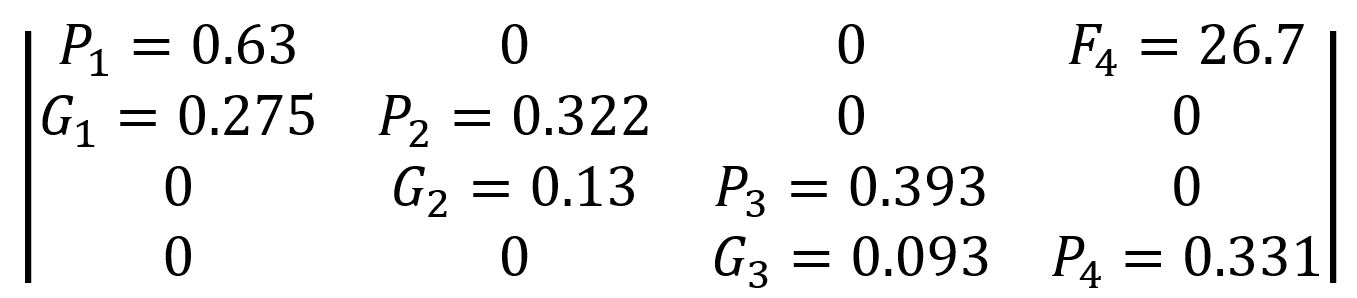
\includegraphics[width=1\linewidth]{MtxFilled} \caption{Stage-based population matrix calculated using Wood's quadratic programming method and parameterized using data from Raberinary and Benbow (2012). \label{WriteMtxRounded}}\label{fig:WriteMtxRounded}
\end{figure}

\hypertarget{model-parameterization}{%
\subsection{Model Parameterization}\label{model-parameterization}}

In order to parameterize this model, we used Wood's Quadratic Programming method (Caswell 2001). Other methods required longer time series than were available to us, were extremely sensitive to noise in the data, or simply resulted in matrices that had no reasonable biological interpretation (Caswell 2001). We estimated a preliminary stage-based matrix model (Figure \ref{WriteMtxRounded}) based on Raberinary and Benbow (2012) data and calculated using the quadprog package in R (Turlach and Weingessel 2019). Model accuracy was assessed by comparing life history values inferred from the matrix with existing literature on \emph{O. cyanea} life history (Table \ref{LifeHistory}). As all of our values calculated from the matrix fell within the known attributes of this species, we were confident that this model gave an accurate mechanistic description for this population's underlying dynamics.

\hypertarget{model-analysis}{%
\subsection{Model Analysis}\label{model-analysis}}

Eigenvalues (\(\lambda\)) were then calculated from the matrix and future populations can be predicted by multiplying a population vector to incrementally higher powers of our matrix where the power of the matrix corresponds to the time length of the projection. We performed sensitivity analysis on the population matrix and eigenvalues using the r package popbio (Stubben and Milligan 2007). Further, as all of the parameters are scaled to a value between 0 and 1 except \(F_4\), a unit change in these parameters will have a greater proportional effect on the eigenvalue than \(F_4\). To address this, we also conducted elasticity analysis using the popbio package (Stubben and Milligan 2007). This will allow us to identify the groups within this octopus population whose protection will most benefit population growth, essentially creating focus points of conservation. The results of sensitivity and elasticity analysis will be included in the supplementary material. Other life history traits that can be calculated from this matrix are stable stage distribution, reproductive value of each stage, and per-stage survivability. We will also use the R package Rage (Jones et al. 2021) to calculate the age in each stage, life expectancy and longevity, the age and probability of reaching maturity, and generation time of this population. We then used the rage package in R to analyze various life history traits of this matrix, the output of which is included in the supplementary material.

Finally, we calculated the minimum survivability increase necessary per stage to result in an increase of the overall population. We did this by increasing the \(P_i\) and \(G_i\) parameters by increasing percentages in each stage i until the overall eigenvalue (\(\lambda\)) became greater than one.

\hypertarget{management-scenarios}{%
\subsection{Management Scenarios}\label{management-scenarios}}

In order to determine optimal conservation strategies, we altered the survivability of \emph{O. cyanea} by different rates from 0-10\% survival increase of the species. Then, we simulated different closure scenarios for each survival increase, by altering the length of annual closures by month. We then multiplied higher powers of the original matrix during months that were simulated to be ``open fishing'' and then when a closure was simulated, the matrix with increased survival was multiplied to the population for that month. We simulated these different scenarios in order to analyze all combinations of conservation strategies that result in stable \emph{O. cyanea} populations including the three month closure that is currently being instituted.

\begin{table}

\caption{\label{tab:LifeHistory}Existing research and information on the per-stage lifespan of \emph{O. Cyanea}. All existing estimates are from Heukelem (1976), Heukelem (1976), Guard and Mgaya (2003), Humber et al. (2006), Aina (2009). Note: Heukelem and Fred (1976) estimate the time to maturity to be 10-13 months (i.e.~stages 1-3 combined). \label{LifeHistory}}
\centering
\begin{tabular}[t]{llrr}
\toprule
Stage & Existing Estimate & Estimate from Lefkovitch Matrix & Variance\\
\midrule
Egg & 20-35 days & NA & NA\\
Larval & 28-56 days & NA & NA\\
1: Immature & No existing estimate & 2.699666 & 4.5885318\\
2: Incipient Maturity & No existing estimate & 1.474724 & 0.7000867\\
3: Mature & No existing estimate & 1.646790 & 1.0651277\\
\addlinespace
4: Fully Mature & No existing estimate & 1.494651 & 0.7393301\\
5: Post Laying & 45-61 days & NA & NA\\
Post larval Phase (stage 1-5) & 9-18 months & NA & NA\\
\bottomrule
\end{tabular}
\end{table}



\hypertarget{results}{%
\section{RESULTS}\label{results}}

The resulting eigenvalue of our matrix was 0.982, indicating a population decline of 1.8\% per month with fishing pressure included (Figure \ref{projection}). The stable stage distribution (Table \ref{lifetable}) shows that 65\% of the makeup of this population is immature individuals, while actively breeding individuals (fully mature) only make up less than 1\% of the naturally occurring population. However, the reproductive output per stage (Table \ref{lifetable}) shows that on average, an individual in this fully mature population is expected to have 41 times the number of offspring as those in stage 1. Larval survivability of 0.0001328 was calculated by dividing our estimated number of larvae surviving back to stage 1 (\(F_4\)) by 201,000 - the average estimated reproductive output of \emph{O. cyanea} by (Guard 2009). The life expectancy of this population was calculated by the Rage package to be 4.06 months with a variance of 5.87 months. The calculated age of maturity is 6.82 months with probability of reaching maturation of 0.022. The longevity of this population (the amount of months for only 1\% of the population to remain) is 12 months with a generation time of 7.38 months.

Changing the survivability of each stage (Figure \ref{stages}) showed that immature individuals (Stage 1) would need the smallest amount (5\%) of survival increase in order to result in overall population growth. Stage 4, on the other hand, would require a survivability increase of 25\% in order to create a viable population.

Our analysis of different closure scenarios (Figure \ref{closures}) indicates closures two months in length or shorter will be ineffective in ensuring a stable population, regardless of how much these closures decreased the death rate of the species. Further, as our baseline growth rate was close to stable (-0.0184), it took a maximum of a 7.5\% increase in the survivability of the population to ensure a sustainable population when utilizing three month closures. This analysis (Figure \ref{closures}) provides all the possible combinations of increased survival rates and frequency of closures that will result in a stable population. Suggested changes in overall survivability range from 2-7.5\%, and the ranges of frequencies of closures span from permanent closure (every month) to once every three months.



\begin{figure}
\centering
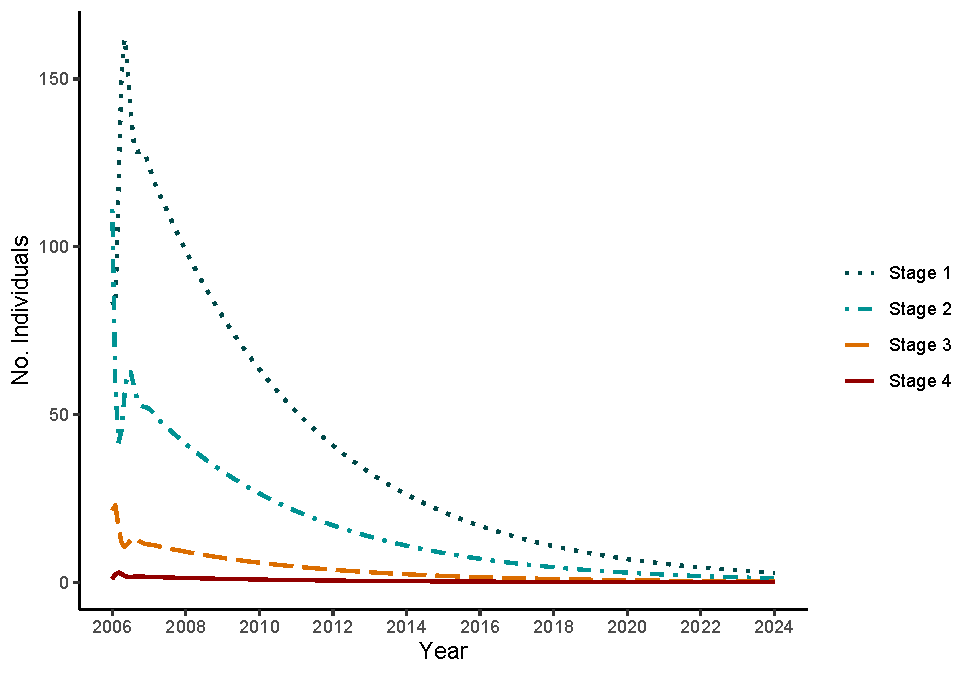
\includegraphics{Wulfing_CH1_Draft4_files/figure-latex/projection-1.pdf}
\caption{\label{fig:projection}Projection of \emph{O. cyanea} population based off of our calculated Lefkovitch matrix through the present. \label{projection}}
\end{figure}

\begin{table}

\caption{\label{tab:lifetable}Stable stage distribution and reproductive value of each stage of this blue octopus population matrix given in Figure \ref{WriteMtxRounded}. The survivability (i.e.~the proportion of individuals who survive from stage i to stage i+1) in each stage includes death rate from fishing. Stages 1-4 survivability were calculated by summing up the proportion of individuals surviving and staying within a stage every month (\(P_i\)) and the proportion of individuals surviving and growing every month (\(G_i\)). Larval survivability of 0.0001328 was calculated by dividing our estimated number of larvae surviving back to stage 1 (\(F_4\)) by the average estimated reproductive output of \emph{O. cyanea}. \label{lifetable}}
\centering
\resizebox{\linewidth}{!}{
\begin{tabular}[t]{l>{\raggedleft\arraybackslash}p{4.5cm}>{\raggedleft\arraybackslash}p{4.5cm}r}
\toprule
Stage & Stable Stage Distribution (Dominant Eigenvector) & Reproductive Value (Left Eigenvector) & Survivability\\
\midrule
1 Immature & 0.657 & 1.000 & 0.9048003\\
2 Incipient Maturity & 0.274 & 1.279 & 0.4519657\\
3 Mature & 0.061 & 6.491 & 0.4859363\\
4 Fully Mature & 0.009 & 41.029 & 0.3309474\\
\bottomrule
\end{tabular}}
\end{table}



\begin{figure}
\centering
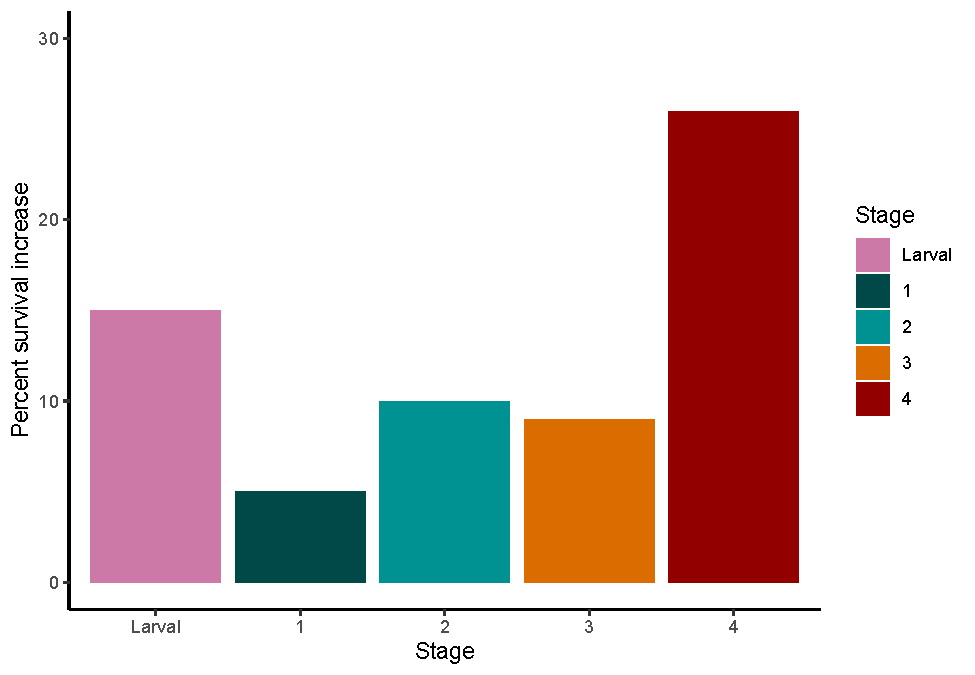
\includegraphics{Wulfing_CH1_Draft4_files/figure-latex/stages-1.pdf}
\caption{\label{fig:stages}Minimum percent of per-stage survivability change needed to create population increase. Each stage was increased by higher percentages until the eigenvalue of the overall system became greater than zero. \label{stages}}
\end{figure}



\begin{figure}
\centering
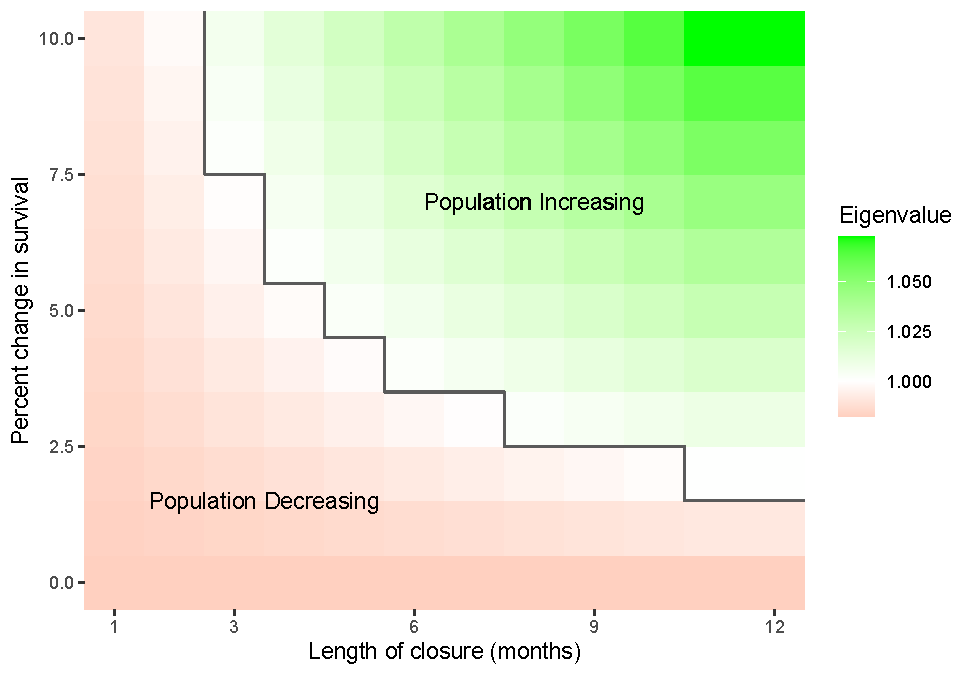
\includegraphics{Wulfing_CH1_Draft4_files/figure-latex/closures-1.pdf}
\caption{\label{fig:closures}Analysis of different management scenarios. The black line separates the scenarios that succeed in sustaining the population from the scenarios that don't. Green and white squares indicate theoretically successful management scenarios where red refers to the strategies that will not result in overall population growth. \label{closures}}
\end{figure}

\hypertarget{discussion}{%
\section{DISCUSSION}\label{discussion}}

Our calculated growth rate of -0.0184 and resulting population projection supports previous reports of overfishing (Humber et al. 2006; Benbow et al. 2014). Decline in population presents an economical issue for individual fishers as their catch will become less lucrative and a recovery of this population will also result in economic gains from fishers in this community (Humber et al. 2006; Benbow et al. 2014; Oliver et al. 2015). Our model provides other information about the life history of this population as well, beyond its overall growth rate. As each column in the matrix represents a proportion of individuals within a stage either growing or staying within a stage (with the exception of the \(F_4\) parameter), it also shows a per-stage survivability estimate (Table \ref{lifetable}) and stage duration (Table \ref{LifeHistory}), life history parameters on which there has been no previous research. However, as the immature stage has a high survivability of 90.4\% and a longer duration than the other stages of 2.7 months, this could indicate that although the fishing method employed in this region does not distinguish by octopus size, fishers may not be bringing this smaller catch to landing due to size limits preventing them from selling immature individuals (Humber et al. 2006). Therefore, this challenges our assumption of the data being properly stratified by size. Further, as \emph{O. Cyanea} have an approximately one to two month larval stage (Guard and Mgaya 2003), the fecundity parameter does not indicate the overall reproductive output of mature individuals, but the number of hatched offspring that will survive its larval stage and back the immature stage. This gives an estimation for larval survivability as female octopus have a fecundity ranging between 27,000 and 375,000 eggs (Guard 2009), our model indicates that only an average of 26.7 individuals will survive back into immaturity, which indicates a survivability of 0.0001328. There is no other larval survivability estimation that currently exists for this species, which would be a useful further study as this could indicate a recruitment rate for this population. Further, an average lifespan of 4.06 months and an age of maturation of 6.82 months indicates that most individuals die before reaching maturation.

Based on our calculations of growth rate over different closure scenarios, any closure less than three months will not be effective in preserving blue octopus stocks, but the strictness of the closure (i.e.~allowing some limited fishing) can be altered depending on how frequently these restricted fishing periods are implemented. There is no literature on the survivability of \emph{O. cyanea} throughout their lifetime, particularly in this region. Therefore, the changes to survivability suggested by our analysis is in relation to their overall death rate not fishing rate, indicating a need for further research on the natural mortality rate of \emph{O. cyanea} before concluding if the three month closure is effective in sustaining fish stocks. Three month closures began to be implemented in the region in 2011 as this length of time was shown to improve octopus yield and had limited negative effects on fisher income (Benbow and Harris 2011). As we don't have a current assessment of \emph{Octopus cyanea} stocks in this fishery, this indicates a need to understand how effective these closures are in preserving the blue octopus of this region. Our analysis of different closure scenarios suggests a range of the simplest actions needed in order to ensure stability of this population. As all combinations of survivability increase and frequency of closure suggested by the analysis will result in stable \emph{O. cyanea} populations, the specific strategy chosen should be decided based on which is most convenient and economically feasible to the local fisher community of southwest Madagascar. Among conservationists, there is a growing understanding that decision making is best left to those directly involved with resource extraction and implementing fishing restrictions upon a community without understanding their cultural practices can have detrimental effects upon the community, as well as be less effective in actually protecting natural resources (Humber et al. 2006; Baker-Médard 2017).

When implemented deliberately, establishing periodic closures is an effective and commonly-used strategy in sustainable fishing practices (Humber et al. 2006; Oliver et al. 2015). As Madagascar has been committed to protecting its marine natural resources through increasing the number of marine parks, this study serves to highlight some of the available strategies to make population predictions and conservation strategies with limited data sources (Westlund 2017). Implementing fishing restrictions without regard for social norms can undermine cultural practices and in turn be detrimental to both the people and fishery, and halts the dissemination of traditional ecological knowledge (Okafor-Yarwood et al. 2022). For this reason, both the Madagascar government and scientific community has found a new emphasis on studying the complex social structures within the community in question in order to more effectively preserve resources along with peoples' livelihoods (Billé and Mermet 2002; Baker-Médard, Gantt, and White 2021). This has been shown to increase participation in conservation practices, therefore making them more effective.

The mechanistic methods used in this study allowed us to gain a baseline understanding of the growth rate and mortality of this population despite the limited data used to parameterize the model. Limitations of this study include the data collection process. Even though daily collections occurred daily within a two-hour window, catch was not standardized by effort and therefore there could be catch fluctuations between months that are not captured in the data. As stage 1 had a high survival rate yet low duration, this challenges the assumption that the octopus caught are an accurate ratio of the octopus at each stage in the wild. Further, matrix population models will converge or diverge based on their dominant eigenvalue, regardless of the initial population inputted in the model. Therefore, we can still conclude that the population at this time was in an overall decline, despite not knowing the exact number of individuals in this population. Another shortcoming of this study is that the only available stage data for this species and region was collected in 2006, and the community of southwest Madagascar has implemented several strategies since that time to improve the sustainability of their fish stocks in the region (Humber et al. 2006; Raberinary and Benbow 2012). Due to the time of data collection, this study does not reflect the current status of \emph{Octopus cyanea}, but outlines the underlying population dynamics and serves to indicate the need for a more current assessment of \emph{O. cyanea} stocks in the region.

Finally, as we are using a Lefkovitch matrix to simulate population fluctuations, these models inherently make simplifying assumptions about the biology of the study species. For example, these models assume that all individuals within a stage are subject to the same growth and mortality rates. As this study uses data collected from a large geographic range (Raberinary and Benbow 2012), different individuals nesting in different regions may be subject to different selective pressures. Further, this population of blue octopus has been shown to exhibit spatial variability depending on their life stage. Younger individuals tend to live in the shallow inner zone of the reef and larger individuals, who are more able to withstand stronger currents, move to deeper waters for more suitable habitats for nesting (Raberinary 2007). Despite these limitations, the data provided is the best data available for fitting a Lefkovitch matrix to this species. Future extensions of this work could include exploring the dynamics of both sexes in the population (Gerber and White 2014) as male octopus have different growth rates and spatial dynamics (Heukelem 1976). Further, a better understanding of the seasonal breeding dynamics of this population of blue octopus could give better insight into the health of this fishery (White and Hastings 2020). Cephalopod juveniles (a key life stage in understanding future population dynamics) often have two seasonal peaks per year, indicating biannual spawning periods (Humber et al. 2006; Katsanevakis and Verriopoulos 2006). This is related to seasonal fluctuations in temperature, as cephalopod growth is related to environmental temperature (Domain, Jouffre, and Caverivière 2000). However, this relationship is subject to a lot of variation (Heukelem 1976; Herwig et al. 2012). Further, as Madagascar is a tropical climate, this trend may be different in our region of study, as suggested by Raberinary and Benbow (2012), where all life stages of O. cyanea were observed year round, suggesting continuous breeding.

With a short generation time, cephalopod species respond more quickly to new management strategies. Future work on other fished species in the region is necessary to understand the effectiveness of temporary closures. This study also highlights the need for further research into the life history patterns of \emph{Octopus cyanea}. Specifically, studies on the natural mortality rate of this species, both in the larval and benthic stages, could better inform both our model and the greater understanding of how populations of this species grow. Further, a more contemporary study on the status of the octopus fishery of southwest Madagascar will paint a more accurate picture of how this population is faring under the current fishing pressure. These studies can also be used to build off of this one as more in depth data collection could be used to add spatial variability to our model, where we then can evaluate the accuracy of the assumption that every individual within a stage is subject to the same selective pressure. Finally, as the people of southwestern Madagascar are actively taking steps to preserve the health of their fisheries, we hope that studies such as these can serve to facilitate informed decision making when choosing how and when to impose fishing restrictions.

\emph{Acknowledgements} - The authors would like to thank the National Science Foundation for the funding on this project {[}grant number 1923707{]}. We would also like to thank Dr.~Sophie Benbow for not only collecting the data on which paper was written, but also her help in contextualizing research and answering questions about data collection.

\emph{Data Availability} - All supplemental material and code for this project are available at \url{https://github.com/swulfing/OCyanea}. All data used to parameterize this model was collected in Raberinary and Benbow (2012)

\newpage

\textbf{References}

\hypertarget{refs}{}
\begin{CSLReferences}{1}{0}
\leavevmode\vadjust pre{\hypertarget{ref-ainaManagementOctopusFishery2009}{}}%
Aina, Tantely Andriamaharo Ny. 2009. {``Management of Octopus Fishery Off {Southwest} {Madagascar}.''} \emph{United Nations University Fisheries Training Programme, Iceland {[}Final Project}, 39. \url{http://www.unuftp.is/static/fellows/document/tantely09prf.pdf}.

\leavevmode\vadjust pre{\hypertarget{ref-andreModellingClimatechangeinducedNonlinear2010}{}}%
André, Jessica, Malcolm Haddon, and Gretta T. Pecl. 2010. {``Modelling Climate-Change-Induced Nonlinear Thresholds in Cephalopod Population Dynamics: {Climate} Change and Octopus Population Dynamics.''} \emph{Global Change Biology} 16 (10): 2866--75. \url{https://doi.org/10.1111/j.1365-2486.2010.02223.x}.

\leavevmode\vadjust pre{\hypertarget{ref-baker-medardGenderingMarineConservation2017}{}}%
Baker-Médard, Merrill. 2017. {``Gendering {Marine} {Conservation}: {The} {Politics} of {Marine} {Protected} {Areas} and {Fisheries} {Access}.''} \emph{Society \& Natural Resources} 30 (6): 723--37. \url{https://doi.org/10.1080/08941920.2016.1257078}.

\leavevmode\vadjust pre{\hypertarget{ref-baker-medardClassedConservationSocioeconomic2021}{}}%
Baker-Médard, Merrill, Courtney Gantt, and Easton R. White. 2021. {``Classed Conservation: {Socio}-Economic Drivers of Participation in Marine Resource Management.''} \emph{Environmental Science \& Policy} 124 (October): 156--62. \url{https://doi.org/10.1016/j.envsci.2021.06.007}.

\leavevmode\vadjust pre{\hypertarget{ref-barnes-mautheTotalEconomicValue2013}{}}%
Barnes-Mauthe, Michele. 2013. {``The Total Economic Value of Small-Scale Fisheries with a Characterization of Post-Landing Trends: {An} Application in {Madagascar} with Global Relevance.''} \emph{Fisheries Research}, 11.

\leavevmode\vadjust pre{\hypertarget{ref-benbowManagingMadagascarOctopus2011}{}}%
Benbow, Sophie, and Alasdair Harris. 2011. {``Managing {Madagascar}'s Octopus Fisheries. {Proceedingsof} the Workshop on {Octopuscyanea} Fisheries, 5-6 {April} 2011, {Toliara}.''} Blue Ventures Conservation Report.

\leavevmode\vadjust pre{\hypertarget{ref-benbowLessonsLearntExperimental2014}{}}%
Benbow, Sophie, F Humber, Ta Oliver, Kll Oleson, Daniel Raberinary, M Nadon, H Ratsimbazafy, and A Harris. 2014. {``Lessons Learnt from Experimental Temporary Octopus Fishing Closures in South-West {Madagascar}: Benefits of Concurrent Closures.''} \emph{African Journal of Marine Science} 36 (1): 31--37. \url{https://doi.org/10.2989/1814232X.2014.893256}.

\leavevmode\vadjust pre{\hypertarget{ref-bethoneyComparisonDropCamera2019}{}}%
Bethoney, N. David, and Caitlin Cleaver. 2019. {``A {Comparison} of {Drop} {Camera} and {Diver} {Survey} {Methods} to {Monitor} {Atlantic} {Sea} {Scallops} ({Placopecten} Magellanicus) in a {Small} {Fishery} {Closure}.''} \emph{Journal of Shellfish Research} 38 (1): 43. \url{https://doi.org/10.2983/035.038.0104}.

\leavevmode\vadjust pre{\hypertarget{ref-billeIntegratedCoastalManagement2002}{}}%
Billé, Raphaël, and Laurent Mermet. 2002. {``Integrated Coastal Management at the Regional Level: Lessons from {Toliary}, {Madagascar}.''} \emph{Ocean \& Coastal Management} 45 (1): 41--58. \url{https://doi.org/10.1016/S0964-5691(02)00048-0}.

\leavevmode\vadjust pre{\hypertarget{ref-briggs-gonzalezLifeHistoriesConservation2016}{}}%
Briggs-Gonzalez, Venetia, Christophe Bonenfant, Mathieu Basille, Michael Cherkiss, Jeff Beauchamp, and Frank Mazzotti. 2016. {``Life Histories and Conservation of Long‐lived Reptiles, an Illustration with the {American} Crocodile ({Crocodylus} Acutus).''} \emph{Journal of Animal Ecology} 1365 (2656.12723): 12.

\leavevmode\vadjust pre{\hypertarget{ref-campEvaluatingShortOpenings2015}{}}%
Camp, Edward V., Brett T. van Poorten, and Carl J. Walters. 2015. {``Evaluating {Short} {Openings} as a {Management} {Tool} to {Maximize} {Catch}-{Related} {Utility} in {Catch}-and-{Release} {Fisheries}.''} \emph{North American Journal of Fisheries Management} 35 (6): 1106--20. \url{https://doi.org/10.1080/02755947.2015.1083495}.

\leavevmode\vadjust pre{\hypertarget{ref-caswell2001matrix}{}}%
Caswell, H. 2001. \emph{Matrix Population Models: {Construction}, Analysis, and Interpretation}. Matrix Population Models: {Construction}, Analysis, and Interpretation. Sinauer Associates. \url{https://books.google.com/books?id=CPsTAQAAIAAJ}.

\leavevmode\vadjust pre{\hypertarget{ref-catalanSpatialTemporalChanges2006}{}}%
Catalán, I. A., M. T. Jiménez, J. I. Alconchel, L. Prieto, and J. L. Muñoz. 2006. {``Spatial and Temporal Changes of Coastal Demersal Assemblages in the {Gulf} of {Cadiz} ({SW} {Spain}) in Relation to Environmental Conditions.''} \emph{Deep Sea Research Part II: Topical Studies in Oceanography} 53 (11-13): 1402--19. \url{https://doi.org/10.1016/j.dsr2.2006.04.005}.

\leavevmode\vadjust pre{\hypertarget{ref-cinnerInstitutionsCommunitybasedManagement2009}{}}%
Cinner, Joshua E., Andrew Wamukota, Herilala Randriamahazo, and Ando Rabearisoa. 2009. {``Toward Institutions for Community-Based Management of Inshore Marine Resources in the {Western} {Indian} {Ocean}.''} \emph{Marine Policy} 33 (3): 489--96. \url{https://doi.org/10.1016/j.marpol.2008.11.001}.

\leavevmode\vadjust pre{\hypertarget{ref-cohenSustainingSmallscaleFisheries2013}{}}%
Cohen, Philippa J., and Simon J. Foale. 2013. {``Sustaining Small-Scale Fisheries with Periodically Harvested Marine Reserves.''} \emph{Marine Policy} 37 (January): 278--87. \url{https://doi.org/10.1016/j.marpol.2012.05.010}.

\leavevmode\vadjust pre{\hypertarget{ref-crouseStageBasedPopulationModel1987}{}}%
Crouse, Deborah T., Larry B. Crowder, and Hal Caswell. 1987. {``A {Stage}-{Based} {Population} {Model} for {Loggerhead} {Sea} {Turtles} and {Implications} for {Conservation}.''} \emph{Ecology} 68 (5): 1412--23. \url{https://doi.org/10.2307/1939225}.

\leavevmode\vadjust pre{\hypertarget{ref-domainGrowthOctopusVulgaris2000}{}}%
Domain, François, Didier Jouffre, and Alain Caverivière. 2000. {``Growth of {\textless{}}Span Class="nocase"{\textgreater{}}\emph{{Octopus} Vulgaris}{\textless{}}/Span{\textgreater{}} from Tagging in {Senegalese} Waters.''} \emph{Journal of the Marine Biological Association of the United Kingdom} 80 (4): 699--705. \url{https://doi.org/10.1017/S0025315400002526}.

\leavevmode\vadjust pre{\hypertarget{ref-emeryManagementIssuesOptions2016}{}}%
Emery, Timothy J., Klaas Hartmann, and Caleb Gardner. 2016. {``Management Issues and Options for Small Scale Holobenthic Octopus Fisheries.''} \emph{Ocean \& Coastal Management} 120 (February): 180--88. \url{https://doi.org/10.1016/j.ocecoaman.2015.12.004}.

\leavevmode\vadjust pre{\hypertarget{ref-fitahiaHighResolutionMassSpectrometry2018}{}}%
Fitahia, Edda Miray, Mikael Croyal, Christian E. Raheriniaina, Véronique Ferchaud-Roucher, and Hassan Nazih. 2018. {``High-{Resolution} {Mass} {Spectrometry} {Unravels} a {Broad} {Range} of {Bioactive} {Lipid} {Species} in {Octopus} Cyanea and {Loligo} Sp. {By}-Products from {Southwestern} {Madagascar}.''} \emph{Waste and Biomass Valorization} 9 (10): 1787--93. \url{https://doi.org/10.1007/s12649-017-9933-x}.

\leavevmode\vadjust pre{\hypertarget{ref-gerberTwosexMatrixModels2014}{}}%
Gerber, Leah R., and Easton R. White. 2014. {``Two-Sex Matrix Models in Assessing Population Viability: When Do Male Dynamics Matter?''} Edited by Marc Cadotte. \emph{Journal of Applied Ecology} 51 (1): 270--78. \url{https://doi.org/10.1111/1365-2664.12177}.

\leavevmode\vadjust pre{\hypertarget{ref-gharouniSensitivityInvasionSpeed2015}{}}%
Gharouni, A, Ma Barbeau, A Locke, L Wang, and J Watmough. 2015. {``Sensitivity of Invasion Speed to Dispersal and Demography: An Application of Spreading Speed Theory to the Green Crab Invasion on the Northwest {Atlantic} Coast.''} \emph{Marine Ecology Progress Series} 541 (December): 135--50. \url{https://doi.org/10.3354/meps11508}.

\leavevmode\vadjust pre{\hypertarget{ref-gilchristReefFishBiomass2020}{}}%
Gilchrist, Hannah, Steve Rocliffe, Lucy G. Anderson, and Charlotte L. A. Gough. 2020. {``Reef Fish Biomass Recovery Within Community-Managed No Take Zones.''} \emph{Ocean \& Coastal Management} 192 (July): 105210. \url{https://doi.org/10.1016/j.ocecoaman.2020.105210}.

\leavevmode\vadjust pre{\hypertarget{ref-gnanalingamFlexibilityTemporaryFisheries2015}{}}%
Gnanalingam, Gaya, and Chris Hepburn. 2015. {``Flexibility in Temporary Fisheries Closure Legislation Is Required to Maximise Success.''} \emph{Marine Policy} 61 (November): 39--45. \url{https://doi.org/10.1016/j.marpol.2015.06.033}.

\leavevmode\vadjust pre{\hypertarget{ref-govanStatusPotentialLocallymanaged2010}{}}%
Govan, Hugh. 2010. {``Status and Potential of Locally-Managed Marine Areas in the {South} {Pacific}:''} \emph{Munich Personal RePEc Archive} 23828.

\leavevmode\vadjust pre{\hypertarget{ref-grorud-colvertMPAGuideFramework2021}{}}%
Grorud-Colvert, Kirsten, Jenna Sullivan-Stack, Callum Roberts, Vanessa Constant, Barbara Horta e Costa, Elizabeth P. Pike, Naomi Kingston, et al. 2021. {``The {MPA} {Guide}: {A} Framework to Achieve Global Goals for the Ocean.''} \emph{Science (New York, N.Y.)} 373 (6560): eabf0861. \url{https://doi.org/10.1126/science.abf0861}.

\leavevmode\vadjust pre{\hypertarget{ref-guardBiologyFisheriesStatus2009}{}}%
Guard, Martin. 2009. {``Biology and Fisheries Status of Octopus in the {Western} {Indian} {Ocean} and the {Suitability} for Marine Stewardship Council Certification.''} e United Nations Environment Programme.

\leavevmode\vadjust pre{\hypertarget{ref-guardArtisanalFisheryOctopus2003}{}}%
Guard, Martin, and Yunus D. Mgaya. 2003. {``The {Artisanal} {Fishery} for {Octopus} Cyanea {Gray} in {Tanzania}.''} \emph{AMBIO: A Journal of the Human Environment} 31 (7): 528--36. \url{https://doi.org/10.1579/0044-7447-31.7.528}.

\leavevmode\vadjust pre{\hypertarget{ref-herwigUsingAgeBasedLife2012}{}}%
Herwig, Jade N., Martial Depczynski, John D. Roberts, Jayson M. Semmens, Monica Gagliano, and Andrew J. Heyward. 2012. {``Using {Age}-{Based} {Life} {History} {Data} to {Investigate} the {Life} {Cycle} and {Vulnerability} of {Octopus} Cyanea.''} Edited by Sebastian C. A. Ferse. \emph{PLoS ONE} 7 (8): e43679. \url{https://doi.org/10.1371/journal.pone.0043679}.

\leavevmode\vadjust pre{\hypertarget{ref-heukelemGrowthBioenergeticsLifespan1976}{}}%
Heukelem, William F Van. 1976. {``Growth, Bioenergetics, and Life-Span of {Octopus} Cyanea and {Octopus} Maya.''} \emph{A Dissertation Submitted to the Graduate Division of the University of Hawaii in Partial Fulfillment of the Requirements for the Degree of Doctor of Philosophy in Zoology}, 232.

\leavevmode\vadjust pre{\hypertarget{ref-HIDDENHARVESTTheGlobal2012}{}}%
{``Hidden {Harvest}-{The} {Global} {Contribution} of {Capture} {Fisheries}.''} 2012. 66469-GLB. The World Bank. \url{https://documents1.worldbank.org/curated/en/515701468152718292/pdf/664690ESW0P1210120HiddenHarvest0web.pdf}.

\leavevmode\vadjust pre{\hypertarget{ref-hiddinkPredictingEffectsArea2006}{}}%
Hiddink, J. G., T. Hutton, S. Jennings, and M. J. Kaiser. 2006. {``Predicting the Effects of Area Closures and Fishing Effort Restrictions on the Production, Biomass, and Species Richness of Benthic Invertebrate Communities.''} \emph{ICES Journal of Marine Science} 63 (5): 822--30. \url{https://doi.org/10.1016/j.icesjms.2006.02.006}.

\leavevmode\vadjust pre{\hypertarget{ref-humberSeasonalClosuresNoTake2006}{}}%
Humber, F., A. Harris, D. Raberinary, and M. Nadon. 2006. {``Seasonal {Closures} of {No}-{Take} {Zones} to Promote {A} {Sustainable} {Fishery} for {Octopus} {Cyanea} ({Gray}) in {South} {West} {Madagascar}.''} Blue Ventures Conservation Report. \url{https://blueventures.org/publications/seasonal-closures-of-no-take-zones-to-promote-a-sustainable-fishery-for-octopus-cyanea-gray-in-south-west-madagascar/}.

\leavevmode\vadjust pre{\hypertarget{ref-ibanezZoogeographicPatternsPelagic2019}{}}%
Ibáñez, Christian M., Heather E. Braid, Sergio A. Carrasco, David A. López‐Córdova, Gabriela Torretti, and Patricio A. Camus. 2019. {``Zoogeographic Patterns of Pelagic Oceanic Cephalopods Along the Eastern {Pacific} {Ocean}.''} \emph{Journal of Biogeography} 46 (6): 1260--73. \url{https://doi.org/10.1111/jbi.13588}.

\leavevmode\vadjust pre{\hypertarget{ref-jensenLocalManagementHighly2010}{}}%
Jensen, Olaf P., Sofia Ortega-Garcia, Steven J. D. Martell, Robert N. M. Ahrens, Michael L. Domeier, Carl J. Walters, and James F. Kitchell. 2010. {``Local Management of a {`Highly Migratory Species'}: {The} Effects of Long-Line Closures and Recreational Catch-and-Release for {Baja} {California} Striped Marlin Fisheries.''} \emph{Progress in Oceanography} 86 (1-2): 176--86. \url{https://doi.org/10.1016/j.pocean.2010.04.020}.

\leavevmode\vadjust pre{\hypertarget{ref-rage}{}}%
Jones, Owen R., Patrick Barks, Iain M Stott, Tamora D James, Sam C Levin, William K Petry, Pol Capdevila, et al. 2021. {``Rcompadre and Rage - Two {R} Packages to Facilitate the Use of the {COMPADRE} and {COMADRE} Databases and Calculation of Life History Traits from Matrix Population Models.''} \emph{bioRxiv}, 2021.04.26.441330. \url{https://doi.org/10.1101/2021.04.26.441330}.

\leavevmode\vadjust pre{\hypertarget{ref-katikiroChallengesFacingLocal2015}{}}%
Katikiro, Robert E., Edison D. Macusi, and K. H. M. Ashoka Deepananda. 2015. {``Challenges Facing Local Communities in {Tanzania} in Realising Locally-Managed Marine Areas.''} \emph{Marine Policy} 51 (January): 220--29. \url{https://doi.org/10.1016/j.marpol.2014.08.004}.

\leavevmode\vadjust pre{\hypertarget{ref-katsanevakisSeasonalPopulationDynamics2006}{}}%
Katsanevakis, Stelios, and George Verriopoulos. 2006. {``Seasonal Population Dynamics of {Octopus} Vulgaris in the Eastern {Mediterranean}.''} \emph{ICES Journal of Marine Science} 63 (1): 151--60. \url{https://doi.org/10.1016/j.icesjms.2005.07.004}.

\leavevmode\vadjust pre{\hypertarget{ref-kawakaDevelopingLocallyManaged2017}{}}%
Kawaka, Joan A., Melita A. Samoilys, Michael Murunga, Julie Church, Carolyne Abunge, and George Waweru Maina. 2017. {``Developing Locally Managed Marine Areas: {Lessons} Learnt from {Kenya}.''} \emph{Ocean \& Coastal Management} 135 (January): 1--10. \url{https://doi.org/10.1016/j.ocecoaman.2016.10.013}.

\leavevmode\vadjust pre{\hypertarget{ref-larocheReefFisheriesSurrounding1997}{}}%
Laroche, J., J. Razanoelisoa, E. Fauroux, and M. W. Rabenevanana. 1997. {``The Reef Fisheries Surrounding the South‐west Coastal Cities of {Madagascar}.''} \emph{Fisheries Management and Ecology} 4 (4): 285--99. \url{https://doi.org/10.1046/j.1365-2400.1997.00051.x}.

\leavevmode\vadjust pre{\hypertarget{ref-mayolMadagascarNascentLocally2013}{}}%
Mayol, Tl. 2013. {``Madagascar's Nascent Locally Managed Marine Area Network.''} \emph{Madagascar Conservation \& Development} 8 (2): 91--95. \url{https://doi.org/10.4314/mcd.v8i2.8}.

\leavevmode\vadjust pre{\hypertarget{ref-mcclanahanResponseCoralReef2008}{}}%
McClanahan, T. R. 2008. {``Response of the Coral Reef Benthos and Herbivory to Fishery Closure Management and the 1998 {ENSO} Disturbance.''} \emph{Oecologia} 155 (1): 169--77. \url{https://doi.org/10.1007/s00442-007-0890-0}.

\leavevmode\vadjust pre{\hypertarget{ref-nowlisShortLongtermEffects2000}{}}%
Nowlis, Joshua Sladek. 2000. {``Short- and Long-Term Effects of Three Fishery-Management Tools on Depleted Fisheries.''} \emph{Bulletin of Marine Science} 66 (3): 12.

\leavevmode\vadjust pre{\hypertarget{ref-okafor-yarwoodSurvivalRichestNot2022}{}}%
Okafor-Yarwood, Ifesinachi, Nelly I. Kadagi, Dyhia Belhabib, and Edward H. Allison. 2022. {``Survival of the {Richest}, Not the {Fittest}: {How} Attempts to Improve Governance Impact {African} Small-Scale Marine Fisheries.''} \emph{Marine Policy} 135 (January): 104847. \url{https://doi.org/10.1016/j.marpol.2021.104847}.

\leavevmode\vadjust pre{\hypertarget{ref-oliverPositiveCatchEconomic2015}{}}%
Oliver, Thomas A., Kirsten L. L. Oleson, Hajanaina Ratsimbazafy, Daniel Raberinary, Sophie Benbow, and Alasdair Harris. 2015. {``Positive {Catch} \& {Economic} {Benefits} of {Periodic} {Octopus} {Fishery} {Closures}: {Do} {Effective}, {Narrowly} {Targeted} {Actions} {`{Catalyze}'} {Broader} {Management}?''} Edited by Dennis M. Higgs. \emph{PLOS ONE} 10 (6): e0129075. \url{https://doi.org/10.1371/journal.pone.0129075}.

\leavevmode\vadjust pre{\hypertarget{ref-raberinaryPeriodePontePoulpe2007}{}}%
Raberinary, Daniel. 2007. {``Periode de Ponte Du Poulpe ({Octopus} Cyanea) {D}'{Andavadoaka} Dans La Region Sud Oest de {Madagascar}.''} Blue Ventures Conservation.

\leavevmode\vadjust pre{\hypertarget{ref-raberinaryReproductiveCycleOctopus2012}{}}%
Raberinary, Daniel, and Sophie Benbow. 2012. {``The Reproductive Cycle of {Octopus} Cyanea in Southwest {Madagascar} and Implications for Fisheries Management.''} \emph{Fisheries Research} 125-126 (August): 190--97. \url{https://doi.org/10.1016/j.fishres.2012.02.025}.

\leavevmode\vadjust pre{\hypertarget{ref-rodhouseRoleConsumers1996}{}}%
Rodhouse, P. G., and M. Nigmatullin. 1996. {``Role as Consumers.''} \emph{Royal Society Publishing}, 20. https://doi.org/\url{https://doi.org/10.1098/rstb.1996.0090}.

\leavevmode\vadjust pre{\hypertarget{ref-russNaturalFishingExperiments1998}{}}%
Russ, G. R., and A. C. Alcala. 1998. {``Natural Fishing Experiments in Marine Reserves 1983-1993: Community and Trophic Responses.''} \emph{Coral Reefs (Online)} 17 (4): 383--97. \url{https://doi.org/10.1007/s003380050144}.

\leavevmode\vadjust pre{\hypertarget{ref-santosAssessingImportanceCephalopods2001a}{}}%
Santos, M. B, M. R Clarke, and G. J Pierce. 2001. {``Assessing the Importance of Cephalopods in the Diets of Marine Mammals and Other Top Predators: Problems and Solutions.''} \emph{Fisheries Research} 52 (1-2): 121--39. \url{https://doi.org/10.1016/S0165-7836(01)00236-3}.

\leavevmode\vadjust pre{\hypertarget{ref-popbio}{}}%
Stubben, Chris J., and Brook G. Milligan. 2007. {``Estimating and Analyzing Demographic Models Using the Popbio Package in r.''} \emph{Journal of Statistical Software} 22 (11).

\leavevmode\vadjust pre{\hypertarget{ref-quadprog}{}}%
Turlach, Berwin A., and Andreas Weingessel. 2019. \emph{Quadprog: Functions to Solve Quadratic Programming Problems}. \url{https://CRAN.R-project.org/package=quadprog}.

\leavevmode\vadjust pre{\hypertarget{ref-vannieuwenhoveCrypticDiversityLimited2019}{}}%
Van Nieuwenhove, Annelore Hilde M., Hajaniaina Andrianavalonarivo Ratsimbazafy, and Marc Kochzius. 2019. {``Cryptic Diversity and Limited Connectivity in Octopuses: {Recommendations} for Fisheries Management.''} Edited by Giacomo Bernardi. \emph{PLOS ONE} 14 (5): e0214748. \url{https://doi.org/10.1371/journal.pone.0214748}.

\leavevmode\vadjust pre{\hypertarget{ref-vaseAcetesKeystoneSpecies2021}{}}%
Vase, Vinaya Kumar, Mohammed K. Koya, Gyanaranjan Dash, Swatipriyankasen Dash, K. R. Sreenath, D. Divu, Rajan Kumar, et al. 2021. {``Acetes as a {Keystone} {Species} in the {Fishery} and {Trophic} {Ecosystem} {Along} {Northeastern} {Arabian} {Sea}.''} \emph{Thalassas: An International Journal of Marine Sciences} 37 (1): 367--77. \url{https://doi.org/10.1007/s41208-020-00276-y}.

\leavevmode\vadjust pre{\hypertarget{ref-wellsObservationsFeedingGrowth1970}{}}%
Wells, M. J., and J. Wells. 1970. {``Observations on the Feeding, Growth Rate and Habits of Newly Settled {\textless{}}Span Class="nocase"{\textgreater{}}\emph{{Octopus} Cyanea}{\textless{}}/Span{\textgreater{}}.''} \emph{Journal of Zoology} 161 (1): 65--74. \url{https://doi.org/10.1111/j.1469-7998.1970.tb02170.x}.

\leavevmode\vadjust pre{\hypertarget{ref-westermanRoleWomenCommunitybased2014}{}}%
Westerman, Kame, and Sophie Benbow. 2014. {``The {Role} of {Women} in {Community}-Based {Small}-{Scale} {Fisheries} {Management}: {The} {Case} of the {South} {West} {Madagascar} {Octopus} {Fishery}.''} \emph{Western Indian Ocean Journal of Marine Science} 12 (2): 119--32.

\leavevmode\vadjust pre{\hypertarget{ref-westlundMarineProtectedAreas2017}{}}%
Westlund, Lena, ed. 2017. \emph{Marine Protected Areas: Interactions with Fishery Livelihoods and Food Security}. Rome: Food; Agriculture Organization of the United Nations.

\leavevmode\vadjust pre{\hypertarget{ref-whiteSeasonalityEcologyProgress2020}{}}%
White, Easton R., and Alan Hastings. 2020. {``Seasonality in Ecology: {Progress} and Prospects in Theory.''} \emph{Ecological Complexity} 44 (December): 100867. \url{https://doi.org/10.1016/j.ecocom.2020.100867}.

\end{CSLReferences}

\end{document}
